\documentclass{ximera}  

\title{Topology}
\author{Melissa Lynn} 
\outcome{Understand the geometry and definitions of open and closed sets. Do very simple proofs about these properties. Identify sets as open, closed, both, or neither.}

\begin{document} 
\begin{abstract}
\end{abstract} 
\maketitle

For many important results and definitions, we'll require domains that have some nice properties. In particular, we'll be concerned with the shapes of our domains. Thinking back to single variable calculus, continuous functions could behave very differently if they were defined on an open interval versus a closed interval.

For example, the extreme value theorem told us that a continuous function on a closed interval $[0,1]$ will always have an absolute maximum and an absolute minimum. However, a continuous function on the open interval $(0,1)$ might not have absolute extrema. The function $f(x) = \frac{1}{x}$ is continuous on $(0,1)$, but has an asymptote $x=0$, and does not have an absolute maximum on the interval $(0,1)$.

ADD GRAPH

On the other hand, open intervals were also important. In order for a limit $\lim_{x\rightarrow C} f(x)$ to exist, the function $f$ needed to be defined on some open interval containing $C$.

We'll need to generalize these concepts of open and closed intervals in order to apply them to multivariable functions. Essentially, we'll need to understand the shapes of our domains. We can do this using ideas from an area of mathematics called ``topology.''

Topology is focused on the shape and spaces, and how to distinguish between different shapes and spaces. However, it takes a much more flexible perspective that you might have seen in geometry classes. In topology, deformations like stretching, shrinking, or bending a space aren't viewed as changing a space. In particular, distance between points isn't important. Instead, topology employs a much looser idea of closeness - provided by open sets, which are a generalization of open intervals.

In general, there are a lot of interesting and weird topological spaces which are not subspaces of any $\mathbb{R}^n$! However, for our purposes, focusing on subspaces of $\mathbb{R}^n$ will be sufficient, so our definitions might look different from some of the definitions you would see in a topology textbook. 

\section*{Open Sets}

You've probably seen many open sets before, without even realizing it! For example, the open interval $(0,1)$ is an open set, as is the disc $\{(x,y)\,|\,x^2+y^2<1\}$ and the open half-plane $\{(x,y)\,|\,x<0\}$.

\begin{image}
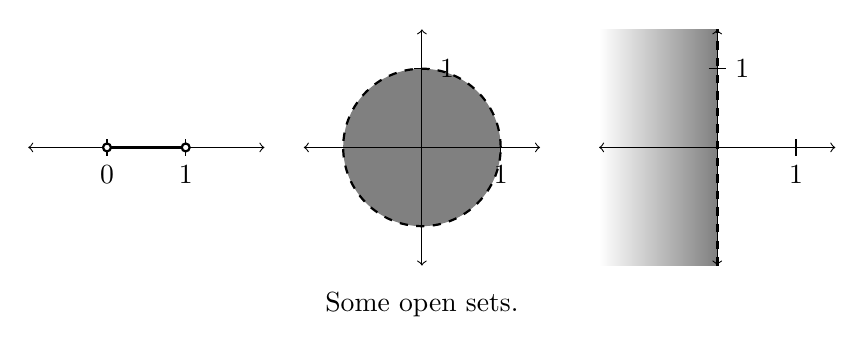
\begin{tikzpicture}
\draw[<->] (-1,0) -- (2,0) ;
\foreach \x in  {0,1}
\draw[shift={(\x,0)},color=black] (0pt,3pt) -- (0pt,-3pt);
\foreach \x in {0,1}
\draw[shift={(\x,0)},color=black] (0pt,0pt) -- (0pt,-3pt) node[below] 
{$\x$};
\node[draw, circle, thick, fill=white, minimum size=1mm, inner sep=0] at (0,0) {};
\node[draw, circle, thick, fill=white, minimum size=1mm, inner sep=0] at (1,0) {};
\draw[very thick] (0.05,0) -- (0.95,0);

\begin{scope}[xshift=4cm]
\node at (0, -2) {Some open sets.};

\draw[thick, dashed, fill=gray] (0,0) circle (1);
\draw[<->] (-1.5,0) -- (1.5,0);
\draw[<->] (0,-1.5) -- (0,1.5);

\foreach \x in {1}
\draw[shift={(\x,0)},color=black] (0pt,3pt) -- (0pt,-3pt) node[below] 
{$\x$};

\foreach \y in {1}
\draw[shift={(0,\y)},color=black] (-3pt,0pt) -- (3pt,0pt) node[right] 
{$\y$};
\end{scope}

\begin{scope}[xshift=7.75cm]
\fill[left color = white,right color = gray]
                (0,-1.5) -- (0,1.5) -- (-1.5,1.5) -- (-1.5, -1.5) --cycle;

\draw[very thick,dashed] (0,-1.5) -- (0,1.5);
\draw[<->] (-1.5,0) -- (1.5,0);
\draw[<->] (0,-1.5) -- (0,1.5);

\foreach \x in {1}
\draw[shift={(\x,0)},color=black] (0pt,3pt) -- (0pt,-3pt) node[below] 
{$\x$};

\foreach \y in {1}
\draw[shift={(0,\y)},color=black] (-3pt,0pt) -- (3pt,0pt) node[right] 
{$\y$};
\end{scope}
\end{tikzpicture}
\end{image}

We begin by defining the most basic type of open set, called an open ball.

\begin{definition}
In $\mathbb{R}^n$, we call $B_r(\mathbf{x})=\{\mathbf{y}\in\mathbb{R}^n\,:\,|\mathbf{x}-\mathbf{y}|<r\}$ the \emph{open ball} of radius $r>0$ centered at $\mathbf{x}$.
\end{definition}

In words, this is the set of points within a fixed distance $r$ of a center point $\mathbf{x}$.


\begin{example}
In $\mathbb{R}^1$, an open ball is simply an open interval. For example, $(1,3)$ is the ball $B_1(2)$ of radius $1$ centered at $2$.

%\begin{image}
%\begin{tikzpicture}
%\draw[<->] (0,0) -- (4,0) ;
%\foreach \x in  {1,2,3}
%\draw[shift={(\x,0)},color=black] (0pt,3pt) -- (0pt,-3pt);
%\foreach \x in {1,2,3}
%\draw[shift={(\x,0)},color=black] (0pt,0pt) -- (0pt,-3pt) node[below] 
%{$\x$};
%\node[draw, circle, thick, fill=white, minimum size=1mm, inner sep=0] at (1,0) {};
%\node[draw, circle, thick, fill=white, minimum size=1mm, inner sep=0] at (3,0) {};
%\draw[very thick] (1.05,0) -- (2.95,0);
%\end{tikzpicture}
%\end{image}

\youtube{QXy9aLiBfSs}


In $\mathbb{R}^2$, an open ball is the inside of a circle (not including the boundary). For example, $B_2((0,3))$ is the inside of the circle of radius $2$ centered at $(0,3)$.

%\begin{image}
%\begin{tikzpicture}
%\draw[thick, dashed, fill=gray] (0,3) circle (2);
%\draw[<->, thick] (-3,0) -- (3,0);
%\draw[<->, thick] (0,-1) -- (0,6);
%
%\foreach \x in {-2,2}
%\draw[shift={(\x,0)},color=black] (0pt,3pt) -- (0pt,-3pt) node[below] 
%{$\x$};
%
%\draw[shift={(0,3)},color=black] (-3pt,0pt) -- (3pt,0pt) node[right] 
%{$3$};
%\end{tikzpicture}
%\end{image}

\youtube{r9OMlNgPqZA}

In $\mathbb{R}^3$, and open ball is the inside of a sphere of radius (not including the boundary). For example, $B_1((0,0,0))$ is the inside of the sphere of radius $1$ centered at the origin.

%\begin{image}
%\begin{tikzpicture}
%  \shade[ball color = gray!40, opacity = 0.4] (0,0) circle (2cm);
%  \draw[thick, densely dotted] (0,0) circle (2cm);
%  \draw[thick, densely dotted] (-2,0) arc (180:360:2 and 0.6);
%  \draw[dashed] (2,0) arc (0:180:2 and 0.6);
%  \fill[fill=black] (0,0) circle (1pt);
%  
%  \draw[<-] (-3, 0) -- (-2,0);
%  \draw[dashed ] (-2,0 ) -- (2,0) node[below, xshift=1ex] 
%{$1$};
%  \draw[->] (2,0) -- (3,0);
%  \draw[<-] (0, -3) -- (0,-2);
%  \draw[dashed] (0,-2 ) -- (0,2) node[right, yshift = 1ex] 
%{$1$};
%  \draw[->] (0,2) -- (0,3);
%  \draw[<-] (-2.5, -1.25) -- (-1,-0.5);
%  \draw[dashed] (-1,-0.5) node[below] 
%{$1$} -- (1.8, 0.9);
%  \draw[->] (1.8, 0.9) -- (2.5, 1.25);
%\end{tikzpicture}
%\end{image}

\youtube{xSHf7KQN6Lc}

\end{example}

In each problem, describe the open ball.

\begin{problem}
In $\mathbb{R}^1$, $B_3(1)$ is the \begin{multipleChoice}
\choice[correct]{open interval}
\choice{inside of a circle}
\choice{inside of a sphere}
\end{multipleChoice}  \begin{problem}$(\answer{-2},\answer{4})$.\end{problem}
\end{problem} 
 
 \begin{problem}
 In $\mathbb{R}^2$, $B_2((1,1))$ is the \begin{multipleChoice}
\choice{open interval}
\choice[correct]{inside of a circle}
\choice{inside of a sphere}
\end{multipleChoice} \begin{problem}of radius $\answer{2}$ centered at $(\answer{1}, \answer{1})$.\end{problem}
\end{problem}

\begin{problem}
In $\mathbb{R}^3$, $B_4((1,2,3))$ is the \begin{multipleChoice}
\choice{open interval}
\choice{inside of a circle}
\choice[correct]{inside of a sphere}
\end{multipleChoice} \begin{problem} of radius $\answer{4}$ centered at $(\answer{1}, \answer{2}, \answer{3})$.\end{problem}
\end{problem}


Now we can define open sets in general, using our new idea of open balls.

\begin{definition}
A set $U\subset \mathbb{R}^n$ is \emph{open} if for every $\mathbf{a}\in U$, there is a radius $r>0$ such that $B_r(\mathbf{a})\subset U$.
\end{definition}

In words, for any point $\mathbf{a}$ in $U$, we can find a radius $r$ small enough that the entire ball of radius $r$ centered at $\mathbf{a}$ is contained in $U$.

%\begin{image}
%\begin{tikzpicture}
%\draw [dashed, fill=gray] plot [smooth cycle] coordinates {(0,0) (2,2) (4,1) (2,-2) (1.5,-0.5)};
%\draw[dashed, fill=darkgray] (2,1.6) circle (.3);
%\draw[fill=black] (2,1.6) circle (.03);
%\end{tikzpicture}
%\end{image}

\youtube{S-cLB6dLCQo}

Even if we don't have an open set, it's possible that there might be some points in $U$ with this special property. We call these interior points.

\begin{definition}
Let $U\subset \mathbb{R}^n$. A point $\mathbf{a}\in U$ is an \emph{interior point} if there is a radius $r>0$ such that $B_r(\mathbf{a})\subset U$.
\end{definition}

So, we can restate the definition of an open set as ``every point is an interior point.''

\begin{problem}

For each of the following, determine whether or not the set is open.

\begin{enumerate}
\item $\{(x,y)\,:\,x^2+y^2<1\}$ in $\mathbb{R}^2$
\begin{multipleChoice}
\choice[correct]{open}
\choice{not open}
\end{multipleChoice}			%VIDEO EXPLANATION
\item $\{(x,y)\,:\,x^2+y^2\leq 1\}$ in $\mathbb{R}^2$
\begin{multipleChoice}
\choice{open}
\choice[correct]{not open}
\end{multipleChoice}			%VIDEO EXPLANATION
\item $\mathbb{R}^2$ in $\mathbb{R}^2$
\begin{multipleChoice}
\choice[correct]{open}
\choice{not open}
\end{multipleChoice}			%VIDEO EXPLANATION
\item $\emptyset$ in $\mathbb{R}^n$
\begin{multipleChoice}
\choice[correct]{open}
\choice{not open}
\end{multipleChoice}			%VIDEO EXPLANATION
\item $\{(x,y)\,:\,x\geq 0\textrm{ and }y\geq 0\}$ in $\mathbb{R}^2$
\begin{multipleChoice}
\choice{open}
\choice[correct]{not open}
\end{multipleChoice}			%VIDEO EXPLANATION
\item $\{(x,y)\,:\,x<y\}$ in $\mathbb{R}^2$
\begin{multipleChoice}
\choice[correct]{open}
\choice{not open}
\end{multipleChoice}			%VIDEO EXPLANATION
\end{enumerate}

\end{problem}

We finish this section by proving an important result about open sets: that the union of a collection of open sets is itself an open set.

\begin{theorem}
Suppose $\{U_i\}$ is a collection of open sets, where each $U_i$ is open. Let $U=\bigcup U_i$, the union of all the $U_i$. Then $U$ is an open set.
\end{theorem}

\begin{proof}
Let $\mathbf{a}\in U$. We will show that $\mathbf{a}$ is an interior point.

Since $\mathbf{a}\in U=\bigcup U_i$, there is some $i$ such that $\mathbf{a}\in U_i$. Since $U_i$ is open, there is a radius $r>0$ such that $B_r(\mathbf{a})$ is contained entirely in $U_i$. Then, since $U_i \subset U$, we have that $B_r(\mathbf{a})\subset U$. This shows that $\mathbf{a}$ is an interior point, and that $U$ is an open set.

%VIDEO EXPLANATION
\end{proof}

\section*{Closed Sets}

We now introduce closed sets, which are defined via their relationship to open sets. Closed sets can be thought of as a generalization of closed intervals.

\begin{definition}
A set $X\subset \mathbb{R}^n$ is \emph{closed} if its complement is open.
\end{definition}

Recall that the \emph{complement} of a subset $X$ of $\mathbb{R}^n$ consists of the elements of $\mathbb{R}^n$ which are not in $X$. That is,
\[
\mathbb{R}^n\setminus X = X^C = \{\mathbf{x}\in\mathbb{R}^n\,:\,\mathbf{x}\in X\}.
\]
$\mathbb{R}^n\setminus X$ and $X^C$ are both common notations for complements. $X^C$ has the advantage of being succinct, while $\mathbb{R}^n\setminus X$ has the advantage of referring to the larger set $\mathbb{R}^n$, which can help avoid confusion.

We now give a couple examples of closed sets.

\begin{example}

The closed interval $[1,3]$ is a closed set in $\mathbb{R}$, since its complement, $(-\infty, 1)\cup (3,\infty)$, is an open set.

The set $\{(x,y)\,:\,x^2+y^2\leq 1\}\subset \mathbb{R}^2$, since its complement, $\{(x,y)\,:\,x^2+y^2> 1\}$, is an open set.

\end{example}

It's very important to remember that, even though closed sets are defined in relation to open sets, {\color{red}``closed'' is not the same as ``not open''}. It is possible for a set to be neither closed nor open, and it's possible for a set to be both open and closed.

\begin{example}

The interval $[0,1)$ in $\mathbb{R}$ is neither closed nor open. It is not open, since $0\in [0,1)$ is not an interior point. It is also not closed, because its complement, $(-\infty, 0)\cup [1,\infty)$, is not open ($1$ is not an interior point).

$\mathbb{R}^2$ (in $\mathbb{R}^2$) is both closed and open. We've seen that its open, and we've seen that its complement, $\emptyset$, is also open. Hence $\mathbb{R}^2$ is both open and closed.

\end{example} 

We've used the word ``boundary'' to refer to the ``edge'' of a set. This intuitive idea is useful in working with example, however we do need a rigorous definition of the boundary of a set, which we now give.

\begin{definition}
A point $\mathbf{x}\in\mathbb{R}^n$ is a \emph{boundary point} of a set $X\in \mathbb{R}^n$ if every $B_r(\mathbf{x})$ (for $r>0$) contains both points in $X$ and points not in $X$.

The set of all boundary points of $X$ is called the \emph{boundary} of $X$.
\end{definition}

\begin{example}

The boundary of $\{(x,y)\,:\,x^2+y^2<1\}\subset\mathbb{R}^2$ is $\{(x,y)\,:\,x^2+y^2=1\}$. %VIDEO

The boundary of the interval $(0,1]\subset\mathbb{R}$ is $\{0,1\}$.

\end{example}

From working with examples of open and closed sets, you may have guessed that closed sets tend to contain their boundary points, while open sets do not. This is supported by the following theorem.

\begin{theorem}
A set $X\subset\mathbb{R}^n$ is closed if and only if it contains all of its boundary points.
\end{theorem}

\begin{proof}
If $X$ is closed, then its complement $X^C$ is open. Consider a boundary point $x$ of $X$. For any radius $r>0$, $B_r(x)$ contains points in $X$ and points in $X^C$. Since $X^C$ is open, this means that $x\notin X^C$. Thus $x\in X$, as desired.

Working in the other direction, suppose that $X$ contains all of its boundary points. We will show that the complement of $X$, $X^C$, is open. Let $x\in X^C$. Since $x$ is not a boundary point of $X$, and any open ball centered at $x$ contains at least one point not in $X$ (namely, $x$), there must be an open ball $B_r(x)$ with $r>0$ containing no points in $X$. Then $B_r(x)\subset X^C$. This shows that $X^C$ is open, and hence $X$ is closed.
\end{proof}

\begin{problem}

For each of the following, determine if the natural domain of the given function is open, closed, both, or neither.

\begin{enumerate}
\item $f(x,y) = \frac{1}{x^2+y^2}$
\begin{multipleChoice}
\choice[correct]{open}
\choice{closed}
\choice{both open and closed}
\choice{neither open nor closed}
\end{multipleChoice}			%VIDEO EXPLANATION
\item $g(x,y) = \sqrt{1-x^2-y^2}$
\begin{multipleChoice}
\choice{open}
\choice[correct]{closed}
\choice{both open and closed}
\choice{neither open nor closed}
\end{multipleChoice}			%VIDEO EXPLANATION
\item $h(x,y) = \frac{1}{\sqrt{1+x^2+y^2}}$
\begin{multipleChoice}
\choice{open}
\choice{closed}
\choice[correct]{both open and closed}
\choice{neither open nor closed}
\end{multipleChoice}			%VIDEO EXPLANATION
\item $a(x,y) = \frac{\sqrt{1-x^2-y^2}}{\sqrt{4}{x^2+y^2-1}}$
\begin{multipleChoice}
\choice{open}
\choice{closed}
\choice[correct]{both open and closed}
\choice{neither open nor closed}
\end{multipleChoice}			%VIDEO EXPLANATION
\item $b(x,y) = \frac{\sqrt[6]{y}}{\sqrt{x}}$
\begin{multipleChoice}
\choice{open}
\choice{closed}
\choice{both open and closed}
\choice[correct]{neither open nor closed}
\end{multipleChoice}			%VIDEO EXPLANATION
\item $c(x,y) = \sqrt{y-x}$
\begin{multipleChoice}
\choice{open}
\choice[correct]{closed}
\choice{both open and closed}
\choice{neither open nor closed}
\end{multipleChoice}			%VIDEO EXPLANATION
\end{enumerate}

\end{problem}

\section*{Neighborhoods}

In calculus, we frequently need to talk about what happens ``near'' or ``close to'' a given point. For example, when defining a limit $\lim_{x\rightarrow a} f(x)$ in single variable calculus, we talk about what happens to $f(x)$ as $x$ \emph{gets close to} $a$. One of the challenges of calculus is figuring out how to make this idea of ``close to'' mathematically rigorous!

One of the ways that we can do this is using neighborhoods, which are really just open sets.

\begin{definition}
Let $\vec{x}\in\mathbb{R}^n$. A \emph{neighborhood} of $\vec{x}$ is an open set $U\subset\mathbb{R}^n$ such that $\vec{x}$ is in $U$.
\end{definition}

Here's the key idea behind talking about neighborhoods: if something happens ``near'' a point, we can find an open set containing that point, where that thing happens. Let's look at some examples.

\begin{example}
If $\vec{x}$ is a point in $\mathbb{R}^n$, and $\vec{y}$ is a different point in $\mathbb{R}^n$, then we can find a neighborhood of $\vec{x}$ that does not contain $\vec{y}$.

We can see why this is true intuitively; if $\vec{x}$ and $\vec{y}$ are different points, then we can draw a tiny little ball around $\vec{x}$ that doesn't contain $\vec{y}$.

\begin{image}
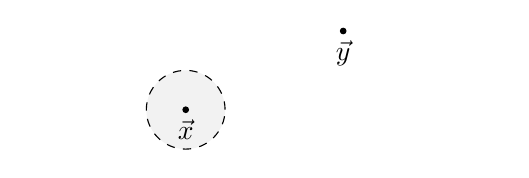
\begin{tikzpicture}
\draw[color = white] (-2,0) -- (4,1);
\draw[dashed, fill = gray!10] (0,0) circle (.5);
\filldraw (0,0) circle (1pt);
\node[anchor=north] at (0,0) {$\vec{x}$};
\filldraw (2,1) circle (1pt);
\node[anchor=north] at (2,1) {$\vec{y}$};
\end{tikzpicture}
\end{image}
\end{example}

\begin{example}
If $\vec{x}$ is a boundary point of a set $U\subset\mathbb{R}^n$, then every neighborhood of $\vec{x}$ contains points in $U$.

We'll draw a picture to see why this is true. If $\vec{x}$ is a boundary point of $U$, then no matter how small we make our neighborhood, it will always contain points from $U$.

\begin{image}
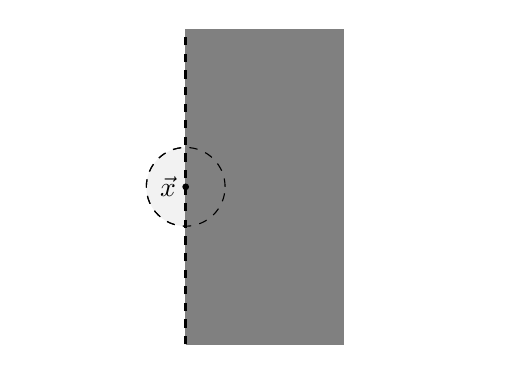
\begin{tikzpicture}
\draw[color = white] (-2,0) -- (4,1);
\draw[dashed, fill = gray!10] (0,0) circle (.5);
\draw[color = gray, fill = gray] (0,-2) -- (0,2) -- (2,2) -- (2,-2) -- (0,-2);
\draw[dashed, very thick] (0,-2) -- (0,2);
\filldraw (0,0) circle (1pt);
\node[anchor=east] at (0,0) {$\vec{x}$};
\draw[dashed] (0,0) circle (.5);
\end{tikzpicture}
\end{image}
\end{example}

As we continue in calculus, you'll frequently come across the phrase ``in a neighborhood of $\vec{x}$.'' Intuitively, this means ``close to $\vec{x}$.'' The precise meaning is, ``in some (possibly very small) open set containing $\vec{x}$.''


\end{document}